\documentclass[11pt,letterpaper]{article}

\usepackage{threeparttable}
\usepackage{textcomp,marvosym}
\usepackage{amsmath,amssymb}
\usepackage[left]{lineno}
\usepackage{changepage}
\usepackage{rotating}
\usepackage{natbib}
\usepackage{setspace}
\usepackage{fancyhdr}
\usepackage{graphicx}
\usepackage{booktabs}
\usepackage{pdfpages}
\usepackage{url}
\usepackage{longtable}
\usepackage{pdflscape}
\usepackage[outercaption]{sidecap}
\doublespacing

\raggedright
\textwidth = 6.5 in
\textheight = 9 in
\oddsidemargin = 0.0 in
\evensidemargin = 0.0 in
\topmargin = 0.0 in
\headheight = 0.0 in
\headsep = 0.0 in
\parskip = 0.1 in
\parindent = 0.2 in

\usepackage[aboveskip=1pt,labelfont=bf,labelsep=period,justification=raggedright,singlelinecheck=off]{caption}

%commands that were used to generate a PDF that was copied to make the .docx version for GSAB
%\pagestyle{empty}
%\usepackage[nomarkers,figuresonly]{endfloat}

\begin{document}

\begin{flushleft}
{\Large \textbf{The Precambrian paleogeography of Laurentia}}
\\

Nicholas L. Swanson-Hysell\textsuperscript{1}

\bigskip

\textsuperscript{1} Department of Earth and Planetary Science, University of California, Berkeley, CA 94720 USA

\end{flushleft}

\noindent\textit{This chapter is in preparation for the book Ancient Supercontinents and the Paleogeography of the Earth}

\linenumbers

\section*{Introduction}

Laurentia was a major continent throughout the majority of the Proterozoic and is hypothesized to have had a central position in both the Paleoproterozoic Nuna and Neoproterozoic Rodinia supercontinents. The paleogeographic position of Laurentia is key to the development of reconstructions of Proterozoic paleogeography. There is a rich record of Precambrian paleomagnetic poles from Laurentia as well as an extensive geologic history of tectonism that are both key to evaluating and developing paleogeographic models. This chapter seeks to provide a concise review of these records.

\section*{Broad tectonic history overview}

Laurentia refers to the craton that forms the Precambrian core of North America (Fig. \ref{fig:Laurentia_map}). Laurentia is comprised of multiple Archean provinces that had unique histories prior to their amalgamation in the Paleoproterozoic, as well as tectonic zones of crustal growth that post-date this assembly \citep{Hoffman1989a, Whitmeyer2007a}. Collision between the Superior province and the composite Slave+Rae+Hearne+Nain provinces that resulted in the Trans-Hudson orogeny represents a major event in the formation of Laurentia \citep{Corrigan2009a}. Terminal collision recorded in the Trans-Hudson orogen is estimated to have been ca. 1.86 to 1.82 Ga based on constraints such as U-Pb dating of monazite grains and zircon rims \citep[e.g.]{Skipton2016a, Weller2017a}. A period of accretionary and collision orogenesis is recorded in the constituent provinces and terranes of Laurentia leading up to the terminal collision of the Trans-Hudson orogeny. This overall story of rapid Paleoproterozoic amalgamation of Laurentia's constituent Archean provinces, including the terminal Trans-Hudson orogeny, was synthesized in the seminal \textit{United Plates of America} paper of \citet{Hoffman1988a} and has been refined in the time since -- particularly with additional geochronological constraints. Of most relevance here are the events that led to the suturing of more major Archean provinces: the Thelon orogen associated with the collision between the Slave province and the Rae province ca. 2.0 to 1.9 Ga \citep{Hoffman1989a}; the Snowbird orogen associated with ca. 1.89 Ga collision between the Rae and Hearne provinces and associated terranes \citep{Berman2007a}; the Nagssugtoqidian orogen due to the ca. 1.86 to 1.84 Ga collision between the Rae and Nain provinces \citep{St-Onge2009a}; and the Torngat orogen resulting from the ca. 1.87 to 1.85 Ga collision of the Meta Incognita province (grouped with the Rae province in older compilations) with the Nain province \citep{St-Onge2009a}. As for the Wyoming province, many models posit that it was conjoined with Hearne and associated provinces at the time of the Trans-Hudson orogeny \citep[e.g.][]{St-Onge2009a, Pehrsson2015a} or was proximal to Hearne and Superior while still undergoing continued translation up to ca. 1.80 Ga \citep{Whitmeyer2007a}. A contrasting view has been been proposed that the Wyoming province and Medicine Hat blocks was not conjoined with the other Laurentia provinces until ca. 1.72 Ga \citep{Kilian2016a}. This interpretation is argued to be consistent with geochronological constraints on monazite and metamorphic zircon indicating active collisional orogenesis associated with the Big Sky orogen on the northern margin of the craton as late as ca. 1.75 to 1.72 Ga \citep{Condit2015a} and ca. 1.72 tectonomagmatic activity in the Black Hills region \citep{Redden1990a}. However, the evidence for earlier orogenesis ca. 1.78 to 1.75 in the Black Hills \citep{Dahl1999a,Hrncir2017a}, as well as high-grade tectonism as early as ca. 1.81 Ga in the Big Sky orogen \citep{Condit2015a}, may support the interpretation of \citet{Hrncir2017a} that ca. 1.72 Ga activity is a minor overprint on ca. 1.75 terminal suturing between Wyoming and Superior. Regardless, in both of these interpretations, Wyoming is a later addition to Laurentia with final suturing post-dating ca. 1.82 Ga amalgamation of Archean provinces with the Trans-Hudson orogen further to the northeast. Overall, the collision of these Archean microcontinents between ca. 1.9 and 1.8 Ga lead to rapid amalgamation of the majority of the Laurentia craton.

\begin{figure}
\centering
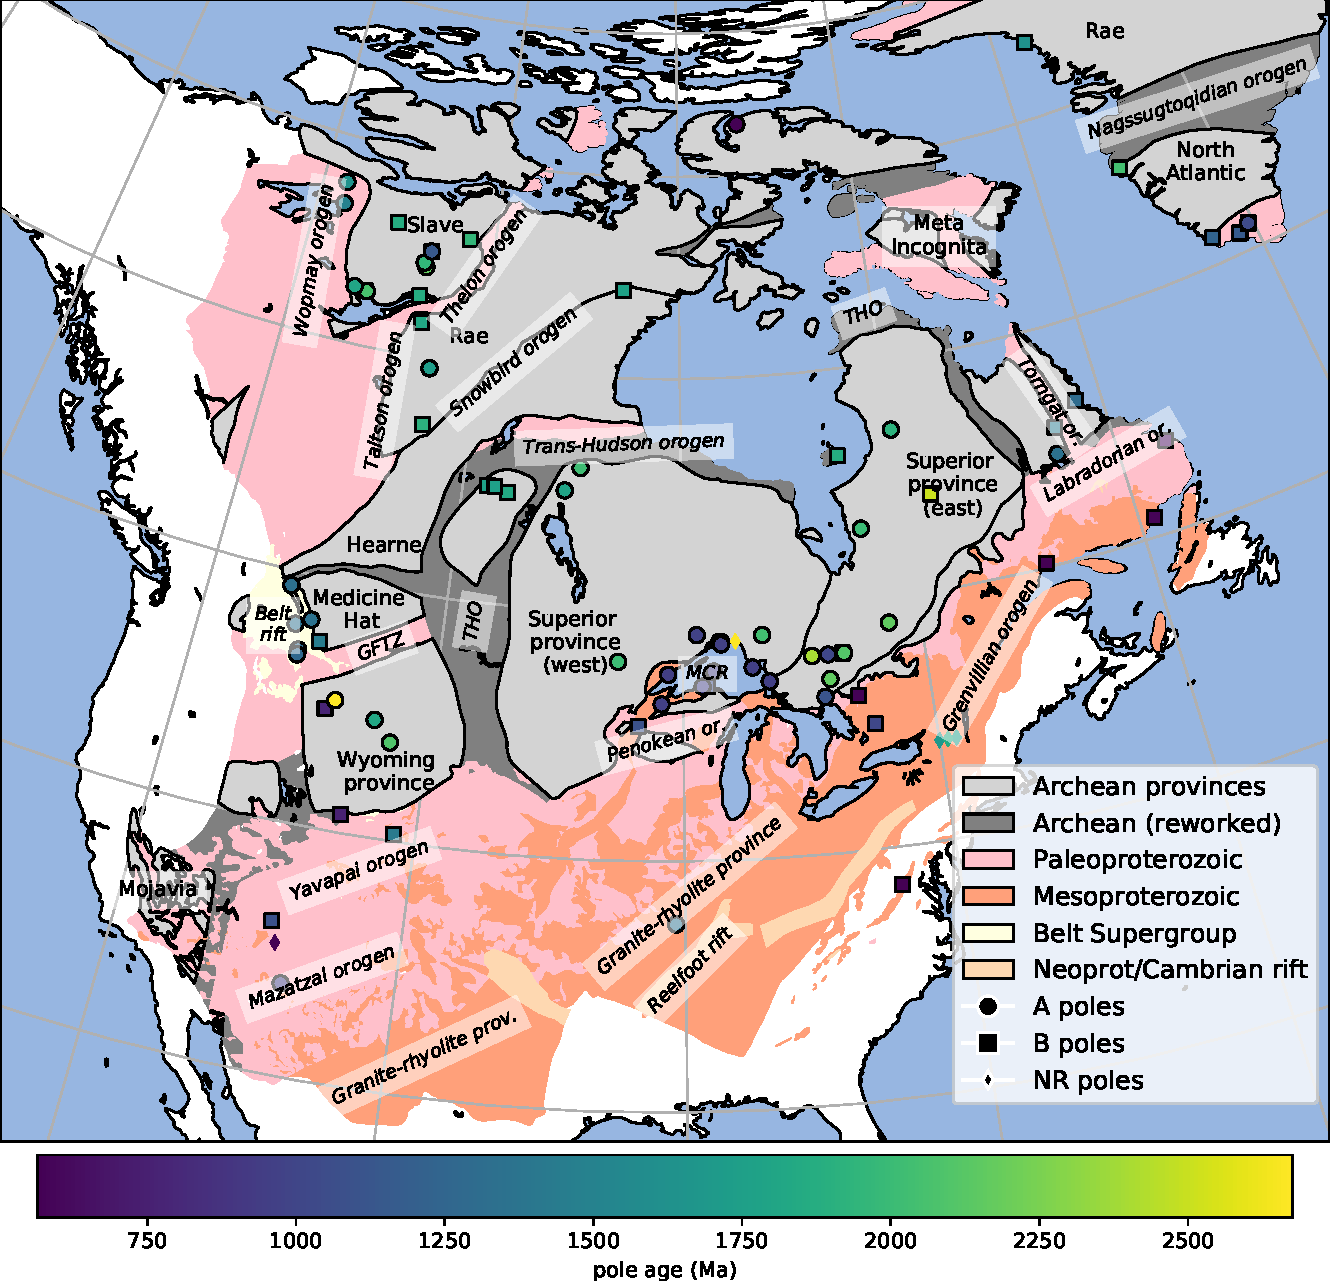
\includegraphics[width=\textwidth]{../Figures/Fig1_map.pdf}
\caption{\small{\textbf{Simplified map of Laurentia showing the location of Archean provinces (labeled with text) and younger Paleoproterozoic and Mesoproterozoic crust (simplified from \citealp{Whitmeyer2007a}). The localities from which the compiled Precambrian paleomagnetic poles were developed are shown and colored by age. The circles (A rated poles) and squares (B rated poles) have been assessed by the Nordic workshop panel while the diamonds are additional not-rated results from the Paleomagia database.}}}
\label{fig:Laurentia_map}
\end{figure} 

Crustal growth also progressed at this time in the Paleoproterozoic through accretionary orogenesis. This accretion occurred within the Wopmay orogen through ca. 1.88 Ga arc-continent collision that led to the accretion of the Hottah terrane (the Calderian orogeny) and the subsequent emplacement of the Great Bear magmatic zone from ca. 1.88 to 1.84 Ga \citep{Hildebrand2009a}. Coeval with the Trans-Hudson orogeny was the perphiral Penokean orogeny on the southern margin of the Superior province with the last evidence of that orogeny being ca. 1.78 undeformed plutons of the East Central Minnesota Batholith \citep{Holm2005a}. 

In the paleogeographic model framework of \cite{Pehrsson2015a}, the collisions of provinces and terranes leading up to the Trans-Hudson orogeny mark the initial phase of assembly of the supercontinent Nuna. The Trans-Hudson orogeny itself is taken to be the terminal collision associated with the closure of the Manikewan Ocean that had previous been a large oceanic tract separating the Superior province from the composite Slave+Rae+Hearne+Nain provinces (often referred to as the Churchill domain or plate; e.g. \citealp{Skipton2016a, Weller2017a}). The \cite{Pehrsson2015a} model posits that this period terminal collision not only resulted in the amalgamation of Laurentia, but is also associated with the assembly of the supercontinent Nuna that is hypothesized to include other major Paleoproterozoic cratons including Siberia, Congo/S\~ao Francisco, West Africa, and Amazonia \citep{Whitmeyer2007a, Pehrsson2015a}. 

Following the Trans-Hudson orogeny, the locus of orogenesis migrated to the exterior of Laurentia. This change marks a shift in the predominant style of Laurentia's growth as subsequent crustal growth occurred dominantly through accretion of juvenile crust along the southern and eastern margin of the nucleus of Archean provinces (\citealp{Whitmeyer2007a}; Figs. \ref{fig:Laurentia_map} and \ref{fig:tectonic_history}). Determining the extent of these belts is complicated by poor exposure of them in the midcontinent relative to the exposure of the Archean provinces throughout the Canadian shield. Major growth of Laurentia following the amalgamation of these Archean provinces occurred associated with the arc-continent collision of the ca. 1.71 to 1.68 Ga Yavapai orogeny. Yavapai orogenesis is interpreted to have resulted from the accretion of a series of arc terranes that collided with each other and Laurentia \citep{Whitmeyer2007a}. Yavapai accretion was followed by widespread emplacement of granitoid intrusions \citep{Whitmeyer2007a}. These intrusions are hypothesized to have stabilized the juvenile accreted terranes that subsequently remained part of Laurentia \citep{Whitmeyer2007a}. Subsequent accretionary orogenesis of the ca. 1.65–1.60 Ga Mazatzal Orogeny and associated plutonism lead to further crustal growth in the latest Paleoproterozoic \citep{Whitmeyer2007a}. Laurentia's growth continued in the Mesoproterozoic along the southeast margin through further juvenile terrane and arc accretion. An interval of major plutonism occurred ca. 1.48–1.35 Ga leading to the formation of A-type granitoids throughout both Mesoproterozoic and Paleoproterozoic provinces extending from the southwest United States up to the Central Gneiss Belt of Ontario to the northeast of Georgian Bay \citep{Slagstad2009a}. This plutonism is likely due to crustal melting within a back-arc region of ca. 1.50 to 1.43 Ga accretionary orogenesis \citep{Bickford2015a}. Younger magmatic activity ca. 1.37 Ga  of the Southern Granite–Rhyolite Province suggests a similar tectonic setting of accretionary orogenesis at that time \citep{Bickford2015a}. While an active margin interpretation with magmatism in back‐arc setting has gained traction within the literature with evidence, the tectonic setting is considered enigmatic given earlier interpretations of an anorogenic setting (see references in \citealp{Slagstad2009a}). 

\begin{figure}
\centering
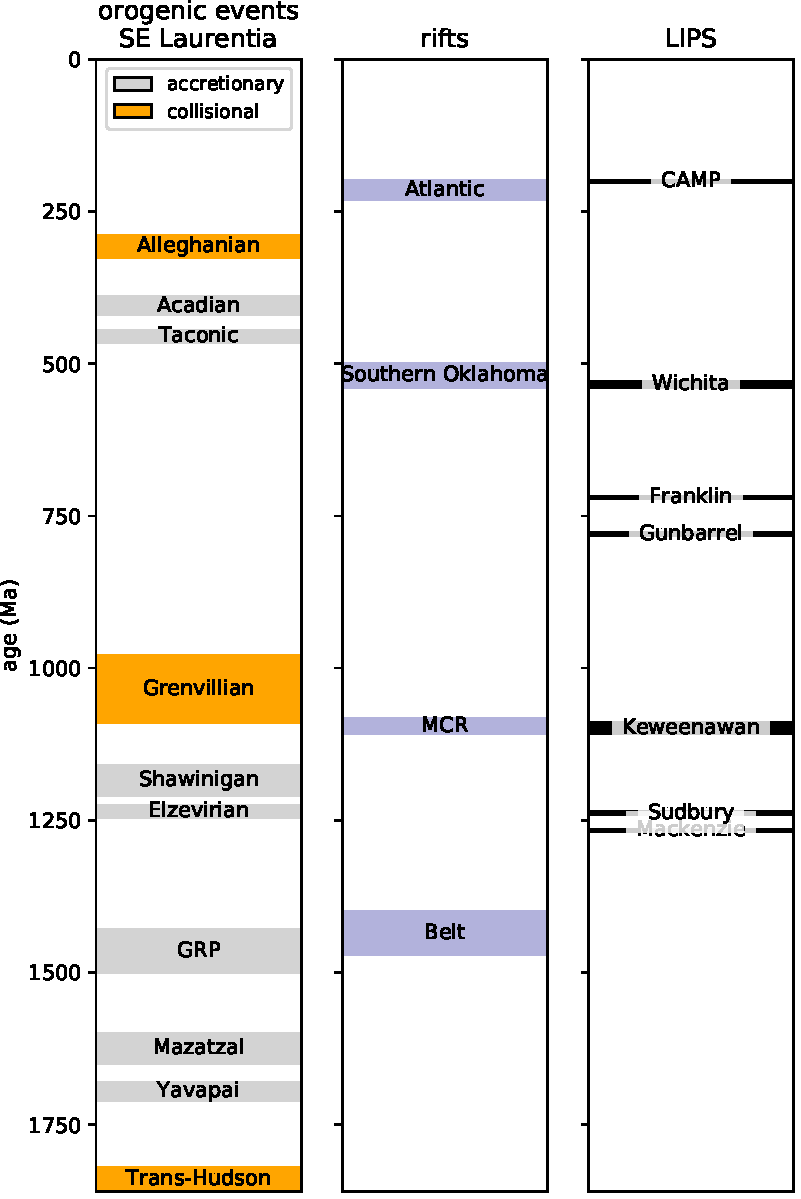
\includegraphics[width=4in]{../Figures/Tectonic_history.pdf}
\caption{\small{\textbf{Simplified summary of Laurentia's tectonic history over the past $\sim$1.8 billion years.} Brief summaries and references related to the orogenic and rifting episodes are given in the text. Note that the Penokean orogeny overlaps with the Trans-Hudson orogeny and is not shown.}}
\label{fig:tectonic_history}
\end{figure}

Accretionary orogenesis continued along the (south)east margin of Laurentia with the arc-continent collision of the ca. 1.25-1.22 Ga Elzevirian orogeny \citep{McLelland2013a}. The subsequent ca. 1.19 to 1.16 Ga Shawinigan orogeny is interpreted to be due to the accretion of a terrane comprised of amalgamated arc volcanics and associated metasediments and is followed by a period of tectonic quiescence on the eastern margin of Laurentia until the collision orogenesis of the Grenvillian orogeny \citep{McLelland2010a}. In the latest Mesoproterozoic (ca. 1.11-1.08 Ga), a major intracontinental rift co-located with a large igneous province formed in Laurentia's interior leading to extension within the Archean Superior province and Paleoproterozoic provinces. This Midcontinent Rift lead to the formation of a thick succession of volcanics and mafic intrusions that are well-preserved in Laurentia's interior.  Midcontinent Rift development ceased as major collisional orogenesis of the Grenvillian orogeny began \citep{Swanson-Hysell2019a}. The Grenvillian orogeny was a protracted interval of continent-continent collision (ca. 1.09 to 0.98 Ga) leading to amphibolite to granulite facies metamorphism through the orogen \citep{McLelland2010a}. The orogeny is interpreted to have resulted in the development of a thick orogenic plateau \citep{Rivers2008a}.

There was significantly less crustal growth on the western margin of Laurentia (Fig. \ref{fig:Laurentia_map}) and the Mesoproterozoic tectonic history is not as well elucidated as on the southern to eastern margin. The 15 to 20 km thick package of sedimentary rocks of the Belt-Purcell Supergroup is associated with ca. 1.47 to 1.40 intracontinental rift -- the tectonic setting of which is debated. \citet{Hoffman1989a} proposed that it may be a remanent back-arc basin trapped within a continent, while others envision it as being associated with continental rifting along the margin associated with separation of a conjugate continent \citep[e.g.]{Jones2015a}. This region is interpreted to have been subsequently deformed during a ca. 1.36 to 1.33 event known as the East Kootenay orogeny \citep{McMechan1982a, Nesheim2012a, McFarlane2015a}. 

This late Paleoproterozoic and Mesoproterozoic tectonic history provides significant constraints on paleogeographic reconstructions. In particular, the long-lived history of accretionary orogenesis along the southeast (present-day coordinates) of Laurentia from the initiation of the Yavapai orogeny (ca. 1.71 Ga) to the end of the Shawinigan orogeny (ca. 1.06 Ga) requires a long-lived open margin without a major conjugate continent up until the time of terminal Grenvillian orogeny collision \citep{Karlstrom2001a}. This constraint is incorporated into models such as that of \citet{Pehrsson2015a} which maintain a long-lived convergent margin throughout the Mesoproterozoic, but in some reconstructions other continental blocks are reconstructed into positions that are seemingly incompatible with this record of accretionary orogenesis (e.g. Amazonia in \citealp{Elming2009a}). The high-grade metamorphism associated with the Ottawan phase of the Grenvillian orogeny itself requires a collision between Laurentia and (an)other continent(s) ca. 1080 Ma -- the geological observation of which first lead to the formulation of the hypothesis of the supercontinent Rodinia \citep{Hoffman1991a}. That the Laurentia margin experienced large-scale continent-continent collision at the time of the Ottawan Phase of the Grenvillian orogeny that is recorded in Texas, up through the Blue Ridge Appalachian inliers, through Ontario and up to the Labrador Sea remains a strong piece of evidence that a supercontinent or (proto)supercontinent formed at the 1.0 Ga Mesoproterozoic to Neoproterozoic transition.

The subsequent Neoproterozoic tectonic history of Laurentia is dominantly a record of rifting. Along the western margin of Laurentia, small-scale rifting occurred ca. 780 to 720 Ma leading to deposition in basins that is recorded from the Death Valley region of SW Laurentia up to the Mackenzie Mountains of NW Laurentia \citep{Rooney2017a}. However, this extensional basin development is relatively minor and predates the more significant rifting that lead to passive margin thermal subsidence that did not occur until the Ediacaran (closer to the ca. 539 Ma Neoproterozoic-Phanerozoic boundary; \citealp{Bond1984a, Levy1991a}). The emplacement of the ca. 780 Ma Gunbarrel large igneous province along this margin and the subsequent extension recorded in the basins is commonly interpreted to be associated with the break-up of Laurentia and a conjugate continent to the western margin. If this interpretation is correct, it is unclear why there would be minimal thermal subsidence until the Ediacaran (post 635 Ma as in \citealp{Levy1991a} and \citealp{Witkosky2018a}). The geological evidence therefore supports active tectonism along the western margin of Laurentia, but suggests that more dramatic lithospheric thinning occurred later than the timing of rifting typically implemented in models of Rodinia break-up. One possibility, along the lines of that proposed in \citet{Ross1991a}, is that ca. 780 Ma extensional tectonism is an inboard record of rifting and passive margin development that occurred further outboard. In this model, subsequent continent rifting that drove lithospheric thinning, perhaps associated with the departure of a microcontinent fragment rather than an already departed major conjugate continent, would be the cause of Ediacaran to Cambrian thermal subsidence. The margin that did experience large-scale rifting and associated passive margin thermal subsidence earlier in the Neoproterozoic is the northeast Greenland margin. Available geochronological constraints and thermal subsidence modeling indicate ca. 820 Ma rifting followed by thermal subsidence of a stable platform \citep{Maloof2006a, Halverson2018a}. These data suggest that conjugate continental lithosphere rifted away from northeast Greenland ca. 820 Ma. 

Extensive rifting that was followed by thermal subsidence occurred along the southeast to east Laurentia margin leading up to the Neoproterozoic-Phanerozoic boundary and is interpreted to be associated with the opening of the Iapetus ocean. A record of this rifting is preserved as rift basins that were part of failed arms (Rome trough, Reelfoot rift and Oklahoma aulacogen) as well as prolonged Cambrian to Ordovician passive margin thermal subsidence along the margin \citep{Bond1984a,Whitmeyer2007a}. The age of igneous intrusions that have been interpreted to be rift-related play a significant role in interpretations of this history such as in the rift development model of \citet{Burton2010a}. In this model, spatially-restricted rifting occurs ca. 760 to 680 Ma in the region of modern-day North Carolina and Virginia. Ca. 620-580 Ma rifting initiates in the region from modern-day New York to Newfoundland and by ca. 580 to 550 Ma rifting extends along the length of Laurentia's eastern margin. The last phases of this rifting are associated with the separation of the Argentine pre-Cordillera Cuyania terrane \citep{Dickerson1998a}. Cuyania is widely interpreted be a rifted fragment of SE Laurentia that separated associated with this early Cambrian rifting and subsequently became part of Gondwana when it collided with other terranes in the vicinity of the Rio de Plata craton during the Ordovician Famatinian orogeny \citep{Martin2019a}. As with other rifts, it is difficult to distinguish the separation of a cratonic fragment as a microcontinent from the rifting of a major craton as the record that lingers on the craton is similar. One interpretation is that there was successful break-up along the eastern margin during the ca. 580 to 550 Ma interval of rifting prior to the ca. 539 Oklahoma aulacogen rifting that liberated the Cuyania microcontinent. The Maz–Arequipa–Rio Apa (MARA) block MARA block with which Cuyania collided \citep{Martin2019a} is likely a product of such rifting. Orogenesis between the MARA block and the Rio de Plata and Kalahari in the ca. 530 Ma Pampean orogeny \citep{Casquet2018a} predated the collision of Cuyania during the ca. 460 Famatinian orogeny. 

The eastern margin of Laurentia then went through the cycle of Appalachian orogenesis. As is visualized in Figure \ref{fig:tectonic_history}, there are parallels between the Grenville orogenic interval and the Appalachian orogenic interval in that there was a period of arc-continent collision (Shawinigan orogeny in the Grenville interval; Taconic orogeny in the Appalachian interval) followed by microcontinent accretion (Llano in the Grenville interval; Acadian in the Appalachian interval) that culminated in large-scale continent-continent collision (Grenvillian orogeny in the Grenville interval; Alleghanian in the Appalachian interval). These similarities are the consequence of an active margin facing an ocean basin that was progressively consumed until its consumption resulted in continent-continent collision. In the case of the Grenville interval, this terminal collision is interpreted to be associated with the assembly of the supercontinent Rodinia and in the Appalachian interval it is interpreted to be associated to with the assembly of the supercontinent Pangea.

Even without considering other continents on Earth, the geological record of Paleoproterozoic collisional of Archean provinces combined with accretionary orogenesis at that time and through the rest of the Paleoproterozoic and Mesoproterozoic provides very strong evidence for mobile plate tectonics driving Laurentia's evolution throughout the past 2 billion years. This tectonic history inferred from geological data can be enhanced through integration with the paleomagnetic record.

\section*{Paleomagnetic pole compilation}

\begin{figure}
\centering
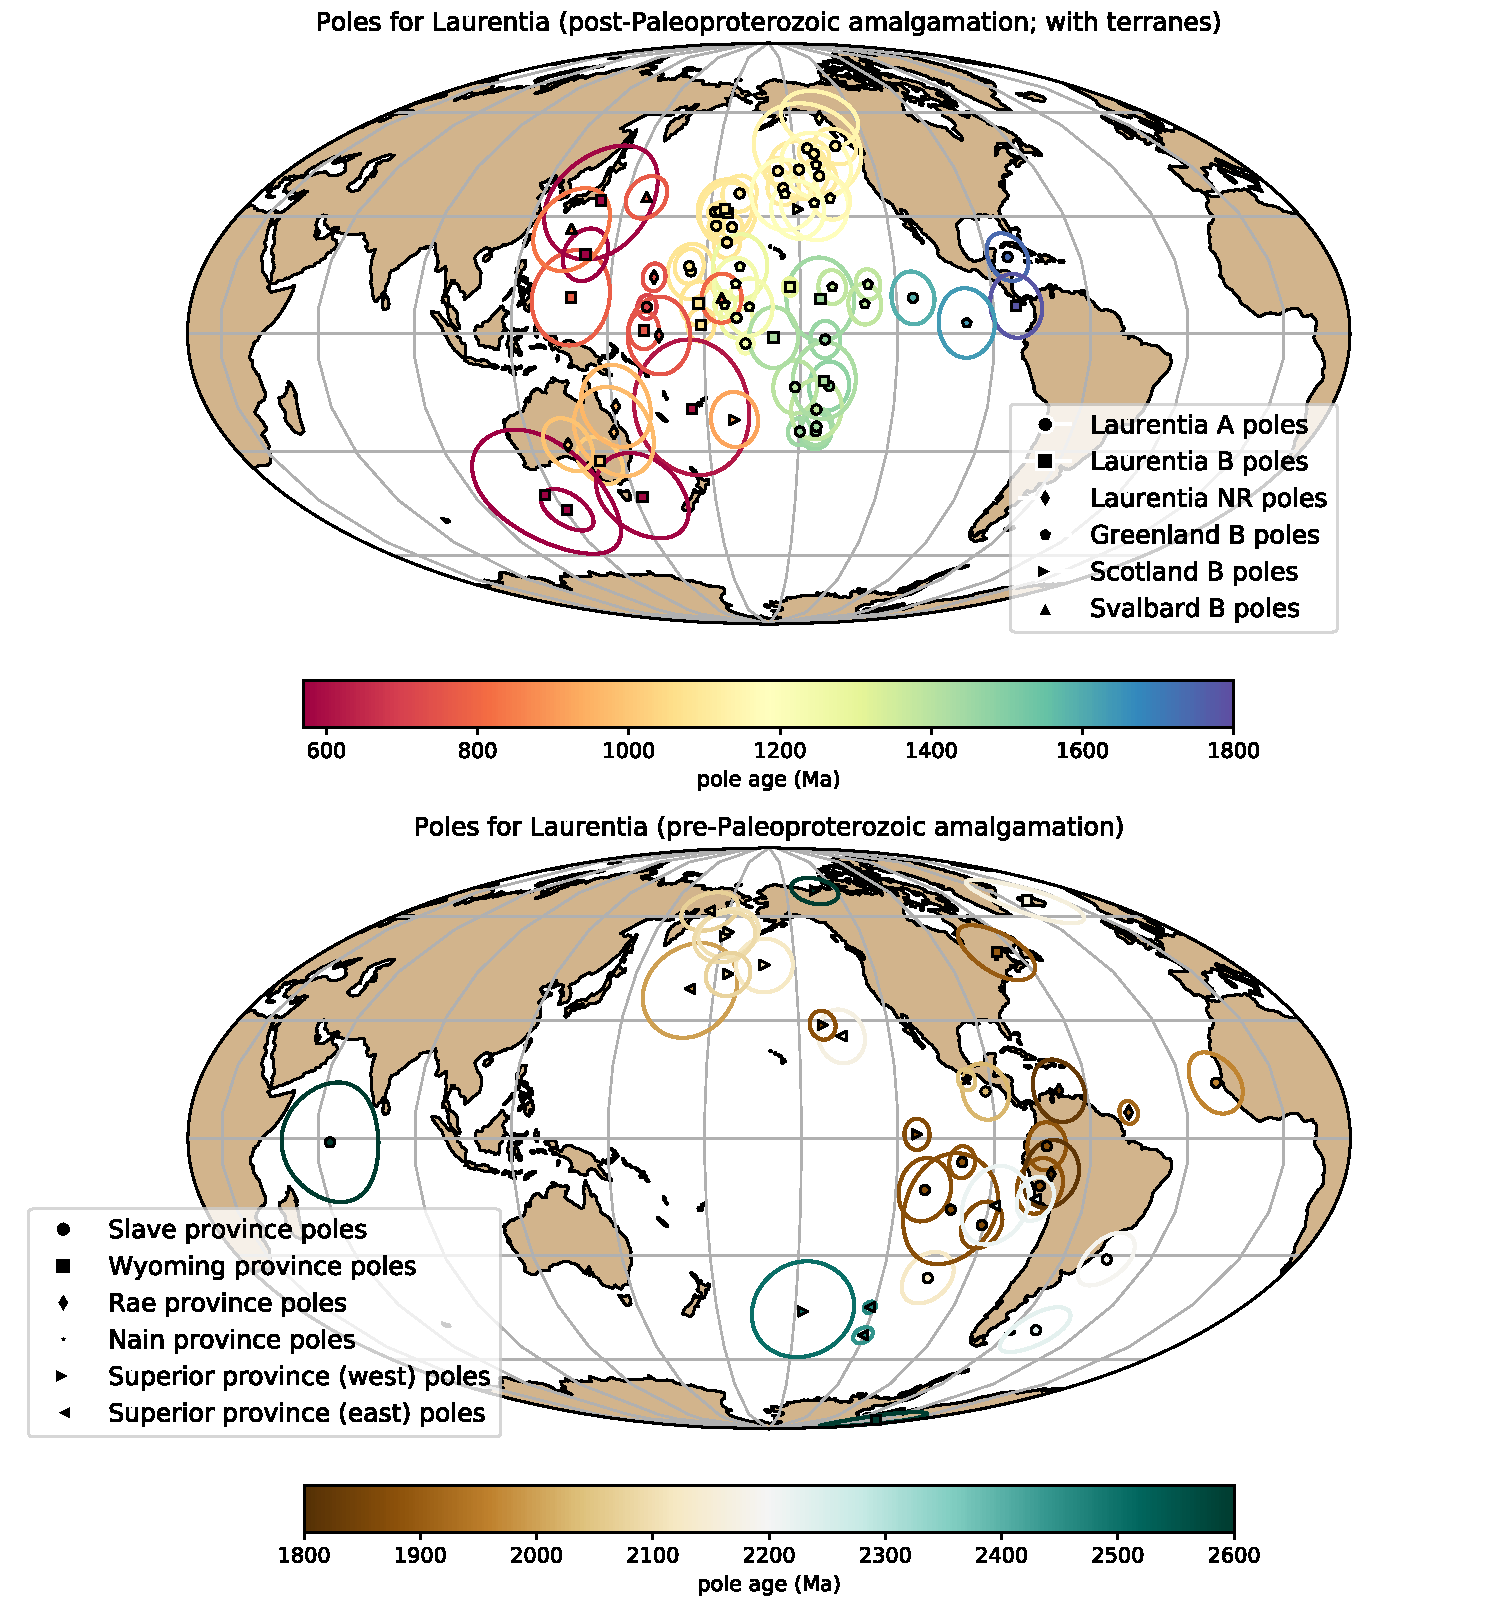
\includegraphics[width=\textwidth]{../Figures/Laurentia_poles_combined.pdf}
\caption{\small{\textbf{Top panel: Paleomagnetic poles from 1800 to 560 Ma for Laurentia (including Greenland, Scotland and Svalbard). Bottom panel: Paleomagnetic data for Archean Provinces prior to the amalgamation of Laurentia.}}}
\label{fig:Laurentia_poles}
\end{figure} 

In this chapter, I focus on the compilation of paleomagnetic poles developed through the Nordic Paleomagnetism Workshops with some additions and modifications. The Nordic Paleomagnetism Workshops have taken the approach of using expert panels to assess paleomagnetic poles and assign them grades meant to convey the confidence that the community has in these results. While many factors associated with paleomagnetic poles can be assessed quantitatively through Fisher statistics and the precision of geochronological constraints, other aspects such as the degree to which available field tests constrain the magnetization to be primary require expert assessment. The categorizations used by the expert panel are `A' and `B' with the last panel meeting occurring in Fall 2017 in Leirubakki, Iceland. An `A' rating refers to poles that are judged to be of such high-quality that they provide essential constraints that should be satisfied in paleogeographic reconstructions. A `B' rating is associated with poles that are judged to likely provide a high-quality constraint, but have some deficiency such as remaining ambiguity in the demonstration of primary remanence or the quality/precision of available geochronologic constraints. Additional poles that were not given an `A' or `B' classification at the Nordic Workshops are referred to as not-rated (`NR'). These additional poles are taken from the Paleomagia database \citep{Veikkolainen2013a}. Many of these poles are quite valuable for reconstruction and should not be dismissed from being considered in paleogeography reconstructions. For example, there are rich data associated with intrusive lithologies of the Grenville Province that are the available paleomagnetic constraints for Laurentia at the Mesoproterozoic-Neoproterozoic boundary. However, the ages of the remanence associated with these poles is complicated by the reality that the magnetization was acquired during exhumation and such cooling ages are more difficult to robustly constrain than for eruptive units or shallow-level intrusions. As a result, the vast majority of Grenville Province poles are not given an `A' or `B' rating. However, while any one of these Grenville poles could be interpreted to suffer from temporal uncertainty, the overall preponderence of poles in a similar location at the time suggests that they need to be taken seriously within any paleogeographic reconstruction of Laurentia (although note an alternative view of an allochthonous origin discussed below). 

Prior to the termination of the Trans-Hudson orogeny (before 1.8 Ga), I consider paleomagnetic poles with respect to the individual Archean provinces. There are poles in the compilation for the Slave, Wyoming, Rae, Superior and Nain provinces prior to Laurentia amalgamation. Overall, these data provide an opportunity to re-evaluate the paleomagnetic evidence for relative motions between Archean provinces prior to Laurentia assembly. A lingering question raised in \citet{Hoffman1988a} that still remains is to what extent the Archean provinces each had independent drift histories with significant separation or whether they have shared histories before experiencing fragmentation and remamalgamation. An analysis of the record strengthened with a new paleomagnetic pole from the Slave province in \cite{Mitchell2014a}, supports significant differential motion between the Superior and Slave provinces between 2.2 and 1.8 Ga. Following the termination of this orogeny (after 1.8 Ga), I consider poles from all the respective provinces and terranes to reflect the position of all of Laurentia. 

For the Superior province, an additional complexity is that paleomagnetic poles from Siderian to Rhyacian Period (2.50 to 2.05 Ga) dike swarms, as well as deflection of dike trends, support an interpretation that there was substantial Paleoproterozoic rotation of the western Superior province relative to the eastern Superior province across the Kapuskasing Structural Zone \citep{Bates1991a, Evans2010a}. This interpretation is consistent with the hypothesis of \citet{Hoffman1988a} that the Kapuskasing Structural Zone represents major intracratonic uplift related to the Trans-Hudson orogeny. \cite{Evans2010a} propose an Euler rotation of (51\textdegree N, 85\textdegree W, -14\textdegree CCW) to reconstruct western Superior relative to eastern Superior and interpret that the rotation occurred in the time interval of 2.07 to 1.87 Ga.  I follow this interpretation and group the poles into Superior (West) and Superior (East). These poles are shown in Table 1 both in their initial reference frame and rotated into the other Superior reference frame. Uncertainty remains with respect to whether the ca. 1.88 Ga Molson dikes pole pre-dates or post-dates this rotation and thus for the time-being should be considered solely in the western Superior province reference frame. 

Following Laurentia's amalgamation, poles from each part of Laurentia can be considered to reflect the position of the entire composite craton. It is worth considering the possibility that poles from zones of Paleoproterozoic and Mesoproterozoic accretion could be allochthonous to the craton. \cite{Halls2015a} argued that this was the case for late Mesoproterozoic and early Neoproterozoic poles from east of the Grenvillian allochthon boundary fault. However, the majority of researchers have considered these poles to post-date major differential motion and be associated with cooling during collapse of a thick orogenic plateau developed during continent-continent collision (e.g. \citealp{Brown2012a}). Poles with a B-rating are also included in the composite that come from Greenland, Svalbard and Scotland. These terranes were once part of contiguous Laurentia, but have subsequently rifted away. These poles need to be rotated into the Laurentia reference frame prior to use for tectonic reconstruction and I apply the  rotations shown in Table \ref{tab:terrane_rotations}.

Through the Proterozoic there are intervals where there are abundant paleomagnetic poles that constrain Laurentia's position and intervals when the record is quite sparse. To visualize the temoporal coverage of the poles and to summarize the motion, implied paleolatitudes for an interior point on Laurentia is shown in Figure \ref{fig:Laurentia_paleolatitude}. There are many high-quality paleomagnetic poles in the early Mesoproterozoic with 12  poles between ca. 1480 and 1380 from Laurentia (including Greenland poles). The best-constrained portion of the record is associated with 1110 to 1083 Ma magmatism within the Midcontinent Rift and southwest Laurentia that enables the development of well-calibrated apparent polar wander path \citep{Swanson-Hysell2019a}. The late Tonian Period also has a number of poles the Gunbarrel LIP (ca. 780 Ma) and Franklin LIP (ca. 720 Ma) as well as contemporaneous sedimentary rocks from western Laurentia basins. Overall the record of paleomagnetic poles has a lot of consistency with progressive paths and agreement between poles. 

%A nice touch would be to add Paleoproterozoic, Meso, Neo and Phanero onto this figure
\begin{figure}
\centering
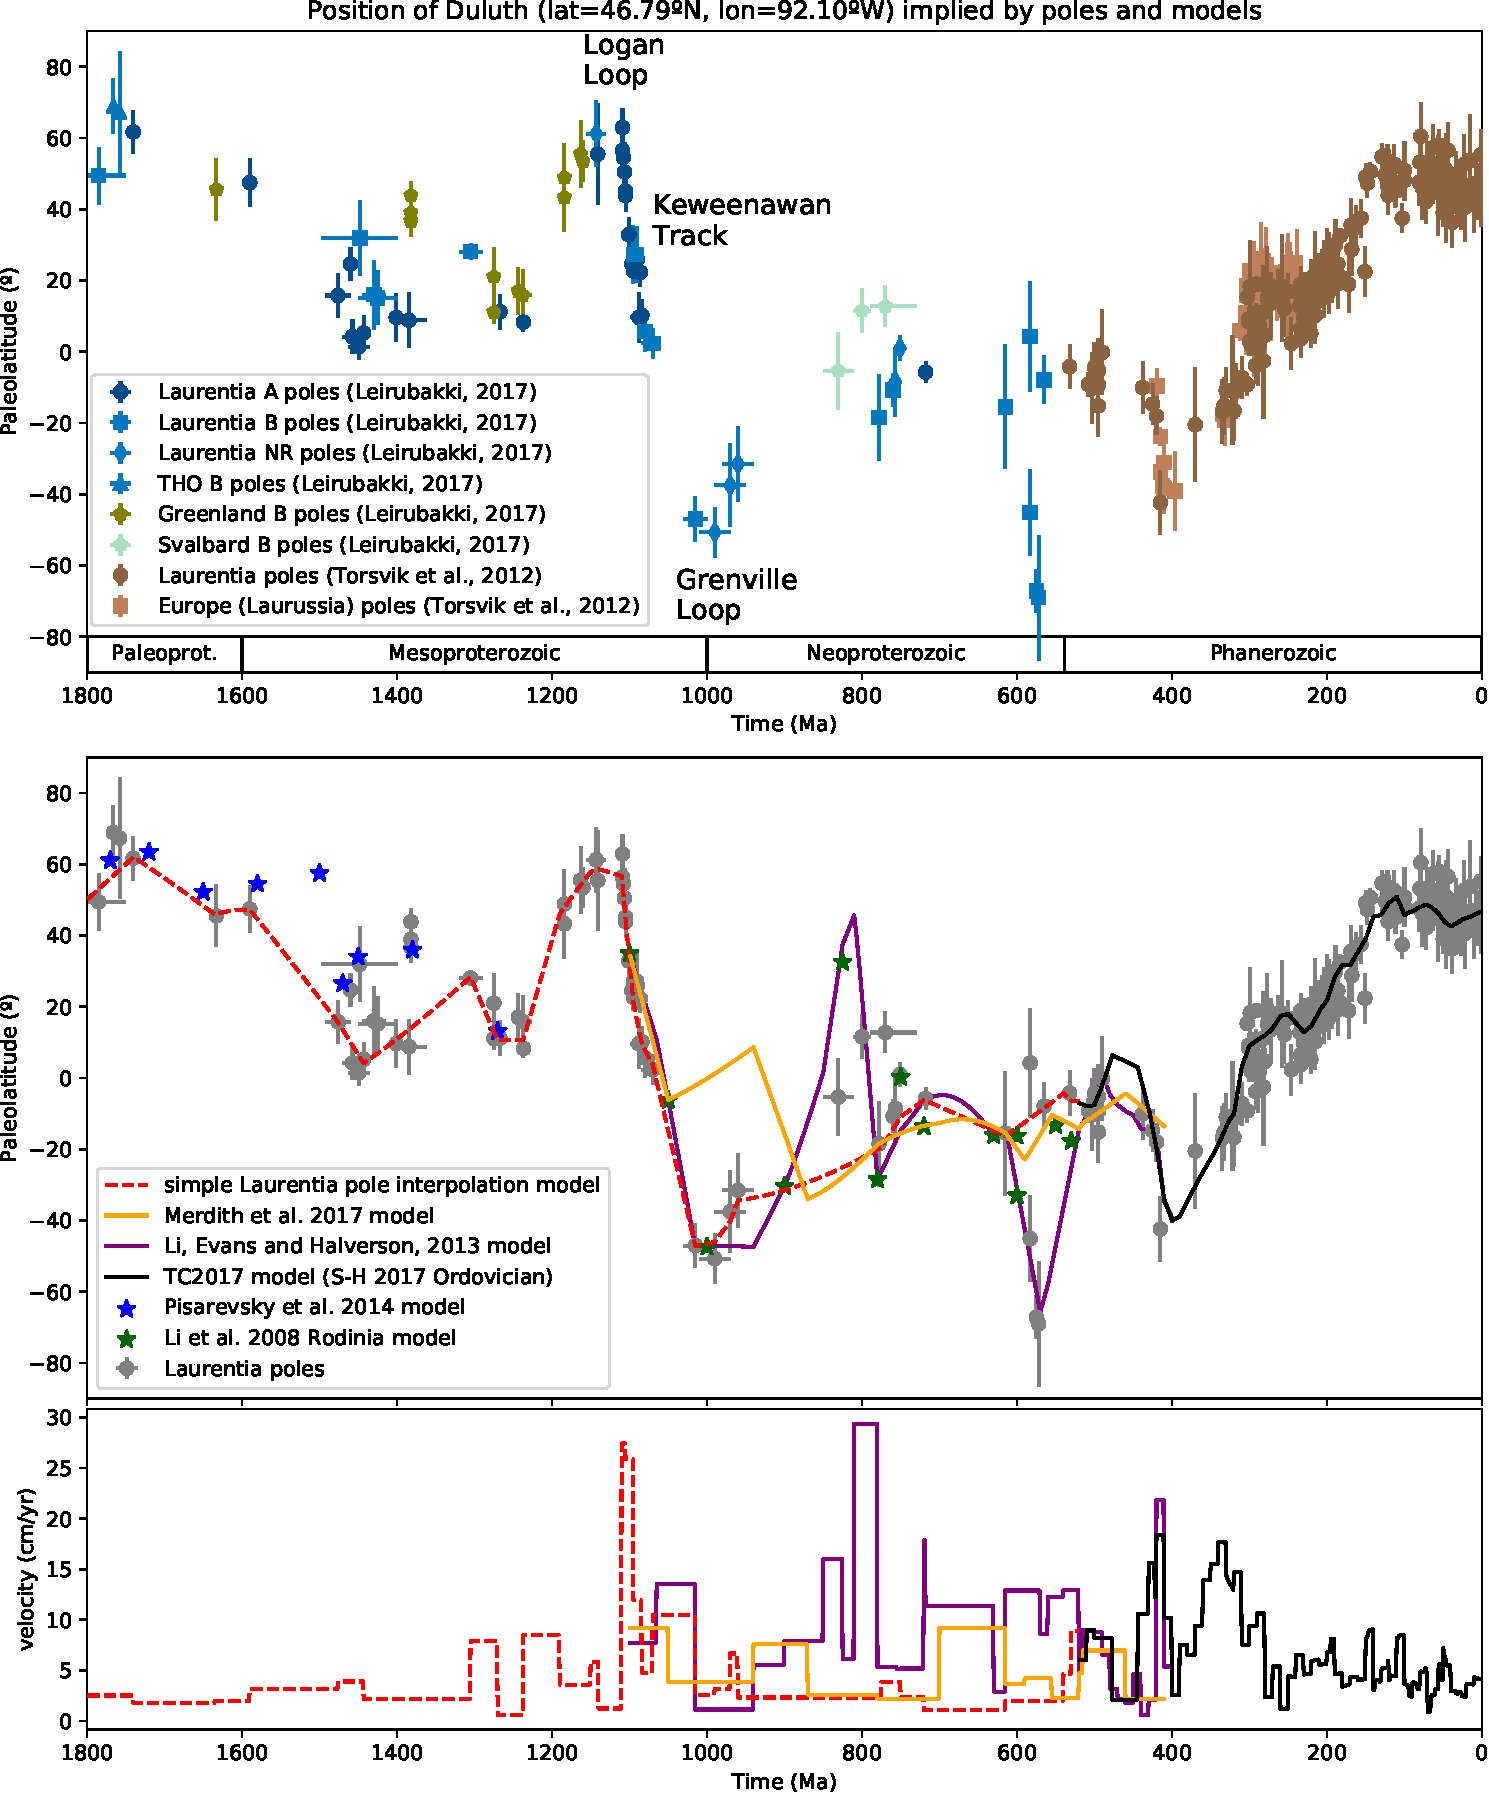
\includegraphics[width=\textwidth]{../Figures/Laurentia_paleolatitude.pdf}
\caption{\small{\textbf{Top panel: Paleolatitude implied by paleomagnetic poles from Laurentia and associated blocks for Duluth (lat=46.79ºN, lon=92.10ºW). The paleomagnetic poles are compiled in Table \ref{tab:Laurentia_poles}. Bottom panel: Paleolatitude implied by Laurentia poles compared with that implied by published paleogeographic models and the simple Laurentia model used in this chapter for the reconstructions in Figure \ref{fig:Laurentia_reconstructions}.}}}
\label{fig:Laurentia_paleolatitude}
\end{figure} 

The combined paleomagnetic poles can be used to develop paleogeographic reconstructions for Laurentia. The method typically applied in the Phanerozoic is to develop synthesized pole paths either through fitting splines through the data or calculating binned running means where the Fisher mean of poles within a given interval are calculated \citep{Torsvik2012}. Such an approach is more challenging when there are significant gaps in the record as is the case through the early Neoproterozoic Era and the late Paleoproterozoic into early Mesoproterozoic.

\section*{Paleogeographic reconstructions}

Seeking to developing comprehensive continuous paleogeographic models is a major challenge given the need to integrate and satisfy diverse geological and paleomagnetic data types. Continually improving constraints related to tectonic setting from improved geologic and geochronologic data need to be carefully integrated with the database of paleomagnetic poles. Paleomagnetic poles compilations themselves are evolving with better data and improved geochronology. Efforts such as this volume are therefore essential to present the state-of-the-art in terms of existing constraints that can be used to evaluate current models and set the stage for future progress.

\begin{figure}
\centering
\includegraphics[width=\textwidth]{../Figures/Laurentia_reconstructions.pdf}
\caption{\small{\textbf{Paleogeogrpahic reconstructions of Laurentia at time intervals through the Proterozoic that are well-constrained by paleomagnetic data. These reconstructions use the simple Laurentia pole interpolation model that is shown in Figure \ref{fig:Laurentia_paleolatitude} and use this model to reconstruct the tectonic elements of \cite{Whitmeyer2007a} shown in Figure \ref{fig:Laurentia_map}. Modern coastlines are maintained in these polygons so that the rotated orientations can be interpreted by the reader in comparison to Figure \ref{fig:Laurentia_map}.}}}
\label{fig:Laurentia_reconstructions}
\end{figure} 

 There is an overall lack of published continuous models in the literature for the Proterozoic that can be compared to the compilation of paleomagnetic poles presented herein. The approach in the community for many years has been to publish models as snapshots at given time intervals presented in figures without publishing continuous rotation parameters. With the further adoption of software tools such as GPlates, there has been significant progress in the publication of continuous paleogeographic models constrained by paleomagnetic poles through the Phanerozoic (540 Ma to present; e.g. \citealp{Torsvik2012a}).
 
 An exception to the paucity of published continuous paleogeographic models for the Precambrian is the Neoproterozoic model of \cite{Merdith2017a} which is shown in comparison to the constraints for Laurentia in Figure \ref{fig:Laurentia_paleolatitude}.  The extent to which the implied position of Laurentia in \cite{Merdith2017a} is consistent with the compiled paleomagnetic constraints can be visualized in Figure \ref{fig:Laurentia_paleolatitude}. As noted above, the development of such models is challenging and the researchers need to balance varying constraints. The focus here will be on the extent to which this model satisfies the available paleomagnetic poles for Laurentia. The model does not honor the Grenville loop (e.g. go to moderately high southerly latitudes ca. 1000 Ma) which is a striking departure from the paleomagnetic record and standard paleogeographic models. Additionally, the implemented plate motion strays from the younger poles of the Keweenawan Track and does not honor the Franklin LIP pole despite its `A' Nordic rating. The Franklin pole is taken to be a key constraint at the Tonian/Cryogenian boundary that provides evidence of the supercontinent Rodinia being equatorial and for the Sturtian glaciation having extended to equatorial latitudes.

There are more published models that show snapshots at given time intervals \cite[e.g.]{Li2008a}.  The synthesis of \citet{Pesonen2012a} developed reconstructions at various Proterozoic time slices.

In this work, I develop a continuous paleogeogrpahic reconstruciton of Laurentia constrained the paleomagnetic poles compilation. This path is based on Laurentia data alone which means that it is poorly constrained through intervals of sparse data (900-800 Ma for example). One could use interpretations of paleogeographic connections with other cratons (e.g. Baltica in the Neoproterozoic) to fill in such portions of the path, however the result then becomes model-dependent without being constrained by data from Laurentia itself. The paleolatitude implied by this continuous model is shown in Figure \ref{fig:Laurentia_paleolatitude}. Paleogeographic snapshots for the past position of Laurentia are shown in Figure \ref{fig:Laurentia_reconstructions.pdf}. These reconstructions use the tectonic elements as defined by \citet{Whitmeyer2007a} with these elements being progressively added associated with Laurentia's growth. As a reminder to the reader, paleomagnetic poles provide constraints on the paleolatitude of a continental block as well as its orientation (which way was north relative to the block). While they provide constraints in this regard, they do not provide constraints in and of themselves to the longitudinal position of the block. Other approaches to obtain paleolongitude utilize geophysical hypotheses such as assuming that large low shear velocity provinces have been stable plume-generating zones in the lower mantle to which plumes can be reconstructed \citep{Torsvik2014a} or that significant pole motion in certain time intervals is associated with true polar wander axes that switch through time in conjunction with the supercontinent cycle \citep{Mitchell2012a}. In Figure \ref{fig:Laurentia_reconstructions.pdf}, Laurentia is centered on the longitudinal position of Duluth with the orientation and paleolatitude being constrained by the paleomagnetic pole compilation as synthesized in the simple Laurentia pole interpolation model.

To make an argument that differential plate tectonic motion began in the Neoproterozoic is to ignore a vast breadth and depth of geological and paleomagnetic data.

\section*{Acknowledgements}

Many participants in the Nordic Paleomagnetism Workshop have contributed to the compilation and evaluation of the pole list utilized herein. Particular acknowledgement goes to David Evans for maintaining and distributing the compiled pole lists as well as additional efforts of Lauri Pesonen in maintining the Paleomagia database \citep{Veikkolainen2014a}. GPlates, and in particular the pyGPlates API, was utilized in this work \citep{Muller2018b}. Figures were made using Matplotlib \citep{Hunter2007a} in conjunction with cartopy \citep{Met-Office2010a} and pmagpy \citep{Tauxe2016a} within an interactive python environment \citep{Perez2007a}. This work was supported by NSF CAREER Grant 1847277 awarded to N.L.S.-H. 

\bibliographystyle{gsabull}
\small\bibliography{../../references/allrefs}


\begin{table}[hbt]
\begin{tabular}{|l|l|l|l|p{2 in}|}
  \hline
& Euler pole & Euler pole & rotation & note and \\
Block & longitude & latitude & angle & citation \\
\hline
Greenland & -118.5 & 67.5 & -13.8 & Cenozoic separation of Greenland from Laurentia associated with opening of Baffin Bay and the Labrador Sea \citep{Roest1989} \\
\hline
Scotland & 161.9 & 78.6 & -31.0 & Reconstructing Atlantic opening following \cite{Torsvik2017a} \\
\hline
Svalbard & 125.0 & -81.0 & 68 & Rotate Svalbard to Laurentia in fit that works well with East Greenland basin according to \cite{Maloof2006a}\\
\hline
\end{tabular}
\caption{}
\end{table}

{\scriptsize
\begin{landscape}
\begin{longtable}{p{1 in}p{1 in}rrrrrrr}
\toprule
                       terrane &                                          unit name & rating &  site lon &  site lat &  plon &  plat &  A$_{95}$ &                    age \\ \hline
\midrule
\endhead
\midrule
\multicolumn{9}{r}{{Continued on next page}} \\ \hline
\midrule
\endfoot

\bottomrule
\endlastfoot
             Laurentia-Wyoming &                            Stillwater Complex - C2 &      A &     249.2 &      45.2 & 335.8 & -83.6 &       4.0 &     2705$^{+4}_{-4}$ \\ \hline
      Laurentia-Superior(East) &                       Otto Stock Dykes and Aureole &      B &     279.9 &      48.0 & 227.0 &  69.0 &       4.8 &     2676$^{+5}_{-5}$ \\ \hline
               Laurentia-Slave &                                       Defeat Suite &      B &     245.5 &      62.5 &  64.0 &  -1.0 &      15.0 &     2625$^{+5}_{-5}$ \\ \hline
      Laurentia-Superior(East) &                                     PTARMIGAN MEAN &      B &     287.0 &      54.0 & 213.0 & -45.3 &      13.8 &     2505$^{+2}_{-2}$ \\ \hline
      Laurentia-Superior(East) &                                       MATACHEWAN R &      A &     278.0 &      48.0 & 238.3 & -44.1 &       1.6 &   2466$^{+23}_{-23}$ \\ \hline
      Laurentia-Superior(East) &                                       MATACHEWAN N &      A &     278.0 &      48.0 & 239.5 & -52.3 &       2.4 &     2446$^{+3}_{-3}$ \\ \hline
               Laurentia-Slave &                                       Malley dykes &      A &     249.8 &      64.2 & 310.0 & -50.8 &       6.7 &     2231$^{+2}_{-2}$ \\ \hline
      Laurentia-Superior(East) &                                         SENNETERRE &      A &     283.0 &      49.0 & 284.3 & -15.3 &       6.0 &     2218$^{+6}_{-6}$ \\ \hline
      Laurentia-Superior(East) &                                       NIPISSING N1 &      A &     279.0 &      47.0 & 272.0 & -17.0 &      10.0 &     2217$^{+4}_{-4}$ \\ \hline
               Laurentia-Slave &                                       Dogrib dykes &      A &     245.5 &      62.5 & 315.0 & -31.0 &       7.0 &     2193$^{+2}_{-2}$ \\ \hline
      Laurentia-Superior(East) &                                        BISCOTASING &      A &     280.0 &      48.0 & 223.9 &  26.0 &       7.0 &     2170$^{+3}_{-3}$ \\ \hline
             Laurentia-Wyoming &    Rabbit Creek, Powder River and South Path Dykes &      A &     252.8 &      43.9 & 339.2 &  65.5 &       7.6 &    2160$^{+11}_{-8}$ \\ \hline
               Laurentia-Slave &                                        Indin dykes &      A &     245.6 &      62.5 & 256.0 & -36.0 &       7.0 &    2126$^{+3}_{-18}$ \\ \hline
      Laurentia-Superior(West) &                                         MARATHON N &      A &     275.0 &      49.0 & 198.2 &  45.4 &       7.7 &     2124$^{+3}_{-3}$ \\ \hline
      Laurentia-Superior(West) &                                         MARATHON R &      A &     275.0 &      49.0 & 182.2 &  55.1 &       7.5 &     2104$^{+3}_{-3}$ \\ \hline
      Laurentia-Superior(West) &                                       CAUCHON LAKE &      A &     263.0 &      56.0 & 180.9 &  53.8 &       7.7 &     2091$^{+2}_{-2}$ \\ \hline
      Laurentia-Superior(West) &                                       FORT FRANCES &      A &     266.0 &      48.0 & 184.6 &  42.8 &       6.1 &     2077$^{+5}_{-5}$ \\ \hline
      Laurentia-Superior(East) &                                         LAC ESPRIT &      A &     282.0 &      53.0 & 170.5 &  62.0 &       6.4 &     2069$^{+1}_{-1}$ \\ \hline
      Laurentia-Greenland-Nain &                                    Kangamiut Dykes &      B &     307.0 &      66.0 & 273.8 &  17.1 &       2.7 &   2042$^{+12}_{-12}$ \\ \hline
               Laurentia-Slave &                                  Lac de Gras dykes &      A &     249.6 &      64.4 & 267.9 &  11.8 &       7.1 &     2026$^{+5}_{-5}$ \\ \hline
      Laurentia-Superior(East) &                                              MINTO &      A &     285.0 &      57.0 & 171.5 &  38.7 &      13.1 &     1998$^{+2}_{-2}$ \\ \hline
               Laurentia-Slave &                    Rifle (Western River) Formation &      B &     252.9 &      65.9 & 341.0 &  14.0 &       7.7 &     1963$^{+6}_{-6}$ \\ \hline
                 Laurentia-Rae &                             Clearwater Anorthosite &      B &     251.6 &      57.1 & 311.8 &   6.5 &       2.9 &     1917$^{+7}_{-7}$ \\ \hline
             Laurentia-Wyoming &                         Sourdough mafic dike swarm &      A &    -108.3 &      44.7 & 292.0 &  49.2 &       8.1 &     1899$^{+5}_{-5}$ \\ \hline
               Laurentia-Slave &                                   Ghost Dike Swarm &      A &     244.6 &      62.6 & 286.0 &  -2.0 &       6.0 &     1887$^{+5}_{-9}$ \\ \hline
               Laurentia-Slave &                           MEAN Seton/Akaitcho/Mara &      B &     250.0 &      65.0 & 260.0 &  -6.0 &       4.0 &     1885$^{+5}_{-5}$ \\ \hline
               Laurentia-Slave &                     MEAN Kahochella, Peacock Hills &      B &     250.0 &      65.0 & 285.0 & -12.0 &       7.0 &     1882$^{+4}_{-4}$ \\ \hline
      Laurentia-Superior(West) &                                        MOLSON B+C2 &      A &     262.0 &      55.0 & 218.0 &  28.9 &       3.8 &     1879$^{+6}_{-6}$ \\ \hline
               Laurentia-Slave &          Douglas Peninsula Formation, Pethei Group &      B &     249.7 &      62.8 & 258.0 & -18.0 &      14.2 &   1876$^{+10}_{-10}$ \\ \hline
               Laurentia-Slave &                                 Takiyuak Formation &      B &     246.9 &      66.1 & 249.0 & -13.0 &       8.0 &   1876$^{+10}_{-10}$ \\ \hline
            Laurentia-Superior &                          MEAN Haig/Flaherty/Sutton &      B &     279.0 &      56.0 & 245.8 &   1.0 &       3.9 &     1870$^{+1}_{-1}$ \\ \hline
               Laurentia-Slave &  MEAN Pearson A/Peninsular sill/Kilohigok basin... &      A &     250.0 &      65.0 & 269.0 & -22.0 &       6.0 &     1870$^{+4}_{-4}$ \\ \hline
 Laurentia-Trans-Hudson orogen &                                Boot-Phantom Pluton &      B &     258.1 &      54.7 & 279.4 &  62.4 &       7.9 &     1838$^{+1}_{-1}$ \\ \hline
                 Laurentia-Rae &                                      Sparrow Dykes &      B &     250.2 &      61.6 & 291.0 &  12.0 &       7.9 &     1827$^{+4}_{-4}$ \\ \hline
                 Laurentia-Rae &                                   Martin Formation &      A &     251.4 &      59.6 & 288.0 &  -9.0 &       8.5 &     1818$^{+4}_{-4}$ \\ \hline
                     Laurentia &                                      Dubawnt Group &      B &     265.6 &      64.1 & 277.0 &   7.0 &       8.0 &   1785$^{+35}_{-35}$ \\ \hline
 Laurentia-Trans-Hudson orogen &                            Deschambault Pegmatites &      B &     256.7 &      54.9 & 276.0 &  67.5 &       7.7 &     1766$^{+5}_{-5}$ \\ \hline
 Laurentia-Trans-Hudson orogen &                                   Jan Lake Granite &      B &     257.2 &      54.9 & 264.3 &  24.3 &      16.9 &     1758$^{+1}_{-1}$ \\ \hline
                     Laurentia &                                      Cleaver Dykes &      A &     242.0 &      67.5 & 276.7 &  19.4 &       6.1 &     1741$^{+5}_{-5}$ \\ \hline
           Laurentia-Greenland &                        Melville Bugt diabase dykes &      B &     303.0 &      74.6 & 273.8 &   5.0 &       8.7 &     1633$^{+5}_{-5}$ \\ \hline
                     Laurentia &                            Western Channel Diabase &      A &     242.2 &      66.4 & 245.0 &   9.0 &       6.6 &     1590$^{+3}_{-3}$ \\ \hline
                     Laurentia &                 St.Francois Mountains Acidic Rocks &      A &     269.5 &      37.5 & 219.0 & -13.2 &       6.1 &   1476$^{+16}_{-16}$ \\ \hline
                     Laurentia &                      Michikamau Intrusion Combined &      A &     296.0 &      54.5 & 217.5 &  -1.5 &       4.7 &     1460$^{+5}_{-5}$ \\ \hline
                     Laurentia &                                  Spokane Formation &      A &     246.8 &      48.2 & 215.5 & -24.8 &       4.7 &   1458$^{+13}_{-13}$ \\ \hline
                     Laurentia &                                 Snowslip Formation &      A &     245.9 &      47.9 & 210.2 & -24.9 &       3.5 &   1450$^{+14}_{-14}$ \\ \hline
                     Laurentia &                    Tobacco Root Dykes - A combined &      B &     247.6 &      47.4 & 216.1 &   8.7 &      10.5 &   1448$^{+49}_{-49}$ \\ \hline
                     Laurentia &                                       Purcell Lava &      A &     245.1 &      49.4 & 215.6 & -23.6 &       4.8 &     1443$^{+7}_{-7}$ \\ \hline
                     Laurentia &                     MEAN Rocky Mountain intrusions &      B &     253.8 &      40.3 & 217.4 & -11.9 &       9.7 &   1430$^{+15}_{-15}$ \\ \hline
                     Laurentia &                                   Mistastin Pluton &      B &     296.3 &      55.6 & 201.5 &  -1.0 &       7.6 &   1425$^{+25}_{-25}$ \\ \hline
                     Laurentia &                                 McNamara Formation &      A &     246.4 &      46.9 & 208.3 & -13.5 &       6.7 &     1401$^{+6}_{-6}$ \\ \hline
                     Laurentia &         Pilcher, Garnet Range and Libby Formations &      A &     246.4 &      46.7 & 215.3 & -19.2 &       7.7 &   1385$^{+23}_{-23}$ \\ \hline
           Laurentia-Greenland &                                Zig-Zag Dal Basalts &      B &     334.8 &      81.2 & 242.8 &  12.0 &       3.8 &     1382$^{+2}_{-2}$ \\ \hline
           Laurentia-Greenland &                              Midsommersoe Dolerite &      B &     333.4 &      81.6 & 242.0 &   6.9 &       5.1 &     1382$^{+2}_{-2}$ \\ \hline
           Laurentia-Greenland &                      Victoria Fjord dolerite dykes &      B &     315.3 &      81.5 & 231.7 &  10.3 &       4.3 &     1382$^{+2}_{-2}$ \\ \hline
                     Laurentia &                                   Nain Anorthosite &      B &     298.2 &      56.5 & 206.7 &  11.7 &       2.2 &   1305$^{+15}_{-15}$ \\ \hline
           Laurentia-Greenland &                                  North Qoroq Intr. &      B &     314.6 &      61.1 & 202.6 &  13.2 &       8.3 &     1275$^{+1}_{-1}$ \\ \hline
           Laurentia-Greenland &                                  Kungnat Ring Dyke &      B &     311.7 &      61.2 & 198.7 &   3.4 &       3.2 &     1275$^{+2}_{-2}$ \\ \hline
                     Laurentia &                         Mackenzie dykes grand mean &      A &     250.0 &      65.0 & 190.0 &   4.0 &       5.0 &     1267$^{+2}_{-2}$ \\ \hline
           Laurentia-Greenland &                         West Gardar Dolerite Dykes &      B &     311.7 &      61.2 & 201.7 &   8.7 &       6.6 &     1244$^{+8}_{-8}$ \\ \hline
           Laurentia-Greenland &                      West Gardar Lamprophyre Dykes &      B &     311.7 &      61.2 & 206.4 &   3.2 &       7.2 &   1238$^{+11}_{-11}$ \\ \hline
                     Laurentia &                             Sudbury Dykes Combined &      A &     278.6 &      46.3 & 192.8 &  -2.5 &       2.5 &     1237$^{+5}_{-5}$ \\ \hline
            Laurentia-Scotland &                                   MEAN Stoer Group &      B &     354.5 &      58.0 & 238.4 &  37.2 &       7.7 &   1199$^{+70}_{-70}$ \\ \hline
           Laurentia-Greenland &                                     Narssaq Gabbro &      B &     313.8 &      60.9 & 225.4 &  31.6 &       9.7 &     1184$^{+5}_{-5}$ \\ \hline
           Laurentia-Greenland &                                 Hviddal Giant Dyke &      B &     313.7 &      60.9 & 215.3 &  33.2 &       9.6 &     1184$^{+5}_{-5}$ \\ \hline
           Laurentia-Greenland &                                  South Qoroq Intr. &      A &     314.6 &      61.1 & 215.9 &  41.8 &      13.1 &     1163$^{+2}_{-2}$ \\ \hline
           Laurentia-Greenland &                                 Giant Gabbro Dykes &      B &     313.7 &      60.9 & 226.1 &  42.3 &       9.4 &     1163$^{+2}_{-2}$ \\ \hline
           Laurentia-Greenland &                          NE-SW Trending Dyke Swarm &      B &     314.6 &      61.1 & 230.8 &  33.4 &       5.7 &     1160$^{+5}_{-5}$ \\ \hline
                     Laurentia &                                      Abitibi Dykes &      A &     279.0 &      48.0 & 215.5 &  48.8 &      14.1 &     1141$^{+2}_{-2}$ \\ \hline
                     Laurentia &                       MEAN Nipigon sills and lavas &      A &     270.9 &      49.1 & 217.8 &  47.2 &       4.0 &     1111$^{+4}_{-4}$ \\ \hline
                     Laurentia &                           Lower Osler volcanics -R &      A &     272.3 &      48.8 & 218.6 &  40.9 &       4.8 &     1108$^{+3}_{-3}$ \\ \hline
                     Laurentia &             Lowermost Mamainse Point volcanics -R1 &      A &     275.3 &      47.1 & 227.0 &  49.5 &       5.3 &     1108$^{+3}_{-3}$ \\ \hline
                     Laurentia &                          Middle Osler volcanics -R &      A &     272.4 &      48.8 & 211.3 &  42.7 &       8.2 &     1107$^{+4}_{-4}$ \\ \hline
                     Laurentia &                           Upper Osler volcanics -R &      A &     272.4 &      48.7 & 201.6 &  42.5 &       3.7 &     1105$^{+2}_{-2}$ \\ \hline
                     Laurentia &                 Lower Mamainse Point volcanics -R2 &      A &     275.3 &      47.1 & 205.2 &  37.5 &       4.5 &     1105$^{+2}_{-2}$ \\ \hline
                     Laurentia &     Mamainse Point volcanics -C (lower N, upper R) &      A &     275.3 &      47.1 & 189.7 &  36.1 &       4.9 &     1101$^{+1}_{-1}$ \\ \hline
                     Laurentia &              Uppermost Mamainse Point volcanics -N &      A &     275.3 &      47.1 & 183.2 &  31.2 &       2.5 &     1098$^{+3}_{-3}$ \\ \hline
                     Laurentia &                               North Shore lavas -N &      A &     268.7 &      46.3 & 181.3 &  34.5 &       2.8 &     1097$^{+3}_{-3}$ \\ \hline
                     Laurentia &                              Chengwatana Volcanics &      B &     267.3 &      45.4 & 186.1 &  30.9 &       8.2 &     1095$^{+2}_{-2}$ \\ \hline
                     Laurentia &                             Portage Lake Volcanics &      A &     271.2 &      47.0 & 178.0 &  26.7 &       4.7 &     1095$^{+3}_{-3}$ \\ \hline
                     Laurentia &                    Cardenas Basalts and Intrusions &      B &     248.1 &      36.1 & 185.0 &  32.0 &       8.0 &     1091$^{+5}_{-5}$ \\ \hline
                     Laurentia &                           Schroeder Lutsen Basalts &      A &     269.1 &      47.5 & 187.8 &  27.1 &       3.0 &     1090$^{+2}_{-7}$ \\ \hline
                     Laurentia &                        Central Arizona diabases -N &      A &     249.2 &      33.7 & 175.3 &  15.7 &       7.0 &   1088$^{+11}_{-11}$ \\ \hline
                     Laurentia &                                   Lake Shore Traps &      A &     271.9 &      47.6 & 186.4 &  23.1 &       4.0 &     1087$^{+2}_{-2}$ \\ \hline
                     Laurentia &                      Michipicoten Island Formation &      A &     274.3 &      47.7 & 174.7 &  17.0 &       4.4 &     1084$^{+1}_{-1}$ \\ \hline
                     Laurentia &                                    Freda Sandstone &      B &     271.5 &      47.0 & 179.0 &   2.2 &       4.2 &   1050$^{+30}_{-30}$ \\ \hline
                     Laurentia &                                     Nonesuch Shale &      B &     271.5 &      47.0 & 178.1 &   7.6 &       5.5 &   1050$^{+30}_{-30}$ \\ \hline
                     Laurentia &                              Haliburton Intrusions &      B &     281.4 &      45.0 & 141.9 & -32.6 &       6.3 &   1015$^{+15}_{-15}$ \\ \hline
            Laurentia-Scotland &                                MEAN Torridon Group &      B &     354.3 &      57.9 & 220.9 & -17.7 &       7.1 &  925$^{+145}_{-145}$ \\ \hline
            Laurentia-Svalbard &                      Lower Grusdievbreen Formation &      B &      18.0 &      79.0 & 204.9 &  19.6 &      10.9 &    831$^{+20}_{-20}$ \\ \hline
            Laurentia-Svalbard &                      Upper Grusdievbreen Formation &      B &      18.2 &      78.9 & 252.6 &  -1.1 &       6.2 &    800$^{+11}_{-11}$ \\ \hline
                     Laurentia &                     MEAN Wyoming "Gunbarrel" dykes &      B &     248.7 &      44.8 & 129.4 &  13.9 &       8.2 &      778$^{+2}_{-2}$ \\ \hline
                     Laurentia &                           Tsezotene Sills Combined &      B &     235.0 &      63.5 & 137.8 &   1.6 &       5.0 &      778$^{+2}_{-2}$ \\ \hline
                     Laurentia &                               Uinta Mountain Group &      B &     250.7 &      40.8 & 161.3 &   0.8 &       4.7 &    775$^{+25}_{-25}$ \\ \hline
            Laurentia-Svalbard &                          Svanbergfjellet Formation &      B &      18.0 &      78.5 & 226.8 &  25.9 &       5.8 &    760$^{+30}_{-30}$ \\ \hline
                     Laurentia &                          Franklin event grand mean &      A &     275.4 &      73.0 & 162.1 &   6.7 &       3.0 &      724$^{+3}_{-3}$ \\ \hline
                     Laurentia &                                   Long Range Dykes &      B &     303.3 &      53.7 & 355.3 &  19.0 &      17.4 &      615$^{+2}_{-2}$ \\ \hline
                     Laurentia &                           Baie des Moutons complex &      B &     301.0 &      50.8 & 321.5 & -34.2 &      15.4 &      583$^{+2}_{-2}$ \\ \hline
                     Laurentia &                           Baie des Moutons complex &      B &     301.0 &      50.8 & 332.7 &  42.6 &      12.0 &      583$^{+2}_{-2}$ \\ \hline
                     Laurentia &                         Callander Alkaline Complex &      B &     280.6 &      46.2 & 301.4 &  46.3 &       6.0 &      575$^{+5}_{-5}$ \\ \hline
                     Laurentia &                                   Catoctin Basalts &      B &     281.8 &      38.5 & 296.7 &  42.0 &      17.5 &      572$^{+5}_{-5}$ \\ \hline
                     Laurentia &                        Sept-Iles Layered Intrusion &      B &     293.5 &      50.2 & 321.0 & -20.0 &       6.7 &      565$^{+4}_{-4}$ \\ \hline
\end{longtable}

\end{landscape}
}

\end{document}